%!TEX root = ../thesis.tex

\section{Introduction}\label{sec:introduction}

Reconstructing character-based phylogenies, which are used to study the evolution of characters shared by a collection of species (taxa or individuals), is a recurring problem in Bioinformatics, mainly due to the complexity of the task. In fact, there exist multiple approaches to evolutionary history reconstruction; most of those approaches try to reduce the problem by limiting the state changes of characters. The Persistent Phylogeny model, which we will talk about in the following sections, allows characters to be acquired and lost at most once in the evolutionary history.

\subsection{Character evolution in Bioinformatics}\label{ssec:charevo}

To study the state changes of characters in an evolutionary tree we can represent species and their characters as rows and columns of a matrix; each element of the matrix marks the specific state of a character for a species.
We will consider the case in which all characters are binary, making them able to assume only one of two states, 0 or 1. For each species, the state of a character represents if the species has or doesn't have a given feature.

\begin{definition}\label{def:m}
  \m{} is a $n \times m$ binary matrix over a set $m$ of characters and a set $n$ of species.

  \m[i][j] represents the state of a character \character[j] for a species \species[i].
\end{definition}

A matrix \m{} can then be represented as an undirected bipartite graph. The set of vertices of the graph is $S \cup C$, where $S$ is the set of species and $C$ the set of characters.

\begin{figure}[h]
  %!TEX root = ../thesis.tex

\begin{subfigure}[b]{0.45\textwidth}
  \centering
    \begin{tabular}{c | c c c c}
      \m{}  & $c_0$ & $c_1$ & $c_2$ & $c_3$ \\ \hline
      $s_0$ & 0     & 1     & 1     & 1     \\
      $s_1$ & 0     & 0     & 0     & 1     \\
      $s_2$ & 1     & 1     & 0     & 0     \\
      $s_3$ & 1     & 0     & 1     & 0
    \end{tabular}

  \caption{Matrix for the instance}\label{figure:1:a}
\end{subfigure}
\hfill
\begin{subfigure}[b]{0.45\textwidth}
  \centering
    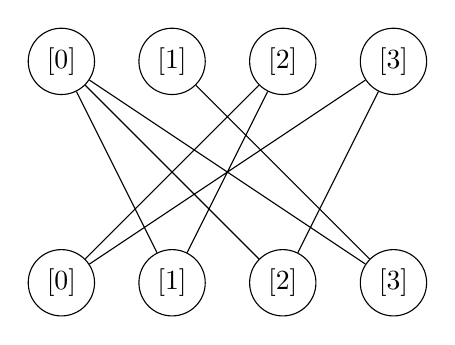
\begin{tikzpicture}
      {\tikzstyle{every node}=[circle, draw]
        \foreach \i in {0, ..., 3}
        {
          \node (s\i) at (\i*40pt, 80pt) {\species[\i]};
        }

        \foreach \j in {0, ..., 3}
        {
          \node (c\j) at (\j*40pt, 0) {\character[\j]};
        }
      }

      \draw
        (c0) -- (s2)
        (c0) -- (s3)
        (c1) -- (s0)
        (c1) -- (s2)
        (c2) -- (s0)
        (c2) -- (s3)
        (c3) -- (s0)
        (c3) -- (s1);
    \end{tikzpicture}

  \caption{Graph for the instance}\label{figure:1:b}
\end{subfigure}


  \caption{An instance of a character-based phylogeny represented as matrix and graph}
  \label{fig:1}
\end{figure}

\subsubsection{Character states}\label{sssec:charstates}

\todo[inline]{Characters can be gained or lost}

Let us introduce the concept of \textit{active} characters.
Active characters \wip{Go on} \dots

\subsection{Persistent Phylogeny problem}\label{ssec:ppp}

\wip[inline]{Add biology PP description \\
             Add PP matrix description}

Each instance of a PPP is associated to a pair \ma{}.

\fix{Sentence start} \dots formalizing input and output parameters for the Persistent Phylogeny problem (PPP) \cite{Bonizzoni2016SolvingTP}.

\begin{definition}[Persistent Phylogeny problem]\label{def:ppp}
  \text{}

  \textit{Input:} pair \ma{} where \m{} is a $n \times m$ binary matrix over a set $m$ of characters and a set $n$ of species, and A is a subset of its characters.

  \textit{Output:} tree $T$ solving \m{} if it exists.
\end{definition}

\subsubsection{Red-black graph representation}\label{sssec:grb}

A red-black graph for an instance of PPP is an undirected bipartite graph whose edges are colored as either red or black.

\begin{definition}[Red-black graph for PPP]\label{def:grb}
  Let $S$ be a set of species vertices, $C$ a set of character vertices, $E$ a set of edges, $A$ a subset of character vertices (active characters).
  Then \grb{} is defined as follows:

  \[ \grb{} = (S, C, E, A) \]

  The vertex set of \grb{} is formally represented as two disjoint and independent sets $S$ and $C$.
\end{definition}

\todo[inline]{GRB and T are in relation thanks to the c-reduction}

A \textit{c-reduction} for a graph \grb{} is the sequence of operations that, when performed on an instance of PPP, clears the graph of all edges.
